
To estimate the number of photoelectrons in the LHC beam pipe, the amount of photons generated by the beam has to be calculated first.
The equations necessary for this were found in~\cite{hofmann}.

Eq.~(5.40) in this reference describes the power spectrum of the radiation emitted by the beam.
\begin{align}
    \derivative{P}{\omega} = \frac{P_s}{\omega_c} S_s(\frac{\omega}{\omega_c})
    \label{eq:dp}
\end{align}
$P_s$ and $\omega_c$ are the total power emitted in the bend and the critical frequency of the radiation:
\begin{align}
    P_s &= \frac{e^2}{4\pi\epsilon_0}\frac{2c\gamma^4}{3\rho^2}
    \label{eq:ps}
    \\
    \omega_c &= \frac{E_c}{\hbar} = \frac{3c\gamma^3}{2\rho}
    \label{eq:omega_c}
    \\
    \frac{P_s}{\omega_c} &= \frac{e^2\gamma}{9\pi\epsilon_0\rho}
\end{align}
An approximation here is $\beta\approx1$, certainly fulfilled for any accelerator that emits significant synchrotron radiation.
The function $S_s$ is an integral over a modified Bessel function.
\begin{align}
    S_s(x) = \frac{9\sqrt{3}}{8\pi} x \int_x^\infty \text{d}z'\ K_{5/3}(z')
    \label{eq:s_s}
\end{align}
The spectrum is easily transformed from frequency to number of photons with the relation $P(\omega)=\dot{n}\hbar\omega$.
Integration yields the number of photons above a certain energy, for example the work function of a material.
\begin{align}
    \derivative{\dot{n}}{\omega} &= \frac{P_s}{\omega_c} \frac{1}{\hbar\omega}S_s(\frac{\omega}{\omega_c})
    \label{eq:nomega}
    \\
    \dot{n} &= \frac{P_s}{E_c}\int_{\omega_\text{min}}^\infty \text{d}\omega \frac{1}{\omega} S_s(\frac{\omega}{\omega_c})
    \\
    &= \frac{P_s}{E_c}\int_{\omega_\text{min}/\omega_c}^\infty \text{d}x \frac{1}{x} S_s(x)
    \\
    &= \underbrace{\frac{P_s}{E_c}  \frac{9\sqrt{3}}{8\pi}}_{=\frac{\sqrt{3}}{8\pi^2\hbar}\frac{e^2\gamma}{\epsilon_0\rho}}
    \cdot
    \underbrace{\int_{\omega_\text{min}/\omega_c}^\infty \text{d}x  \int_x^\infty \text{d}z' K_{5/3}(z')}_{=A(\omega_\text{min}/\omega_c) = A(x_\text{min})}
\end{align}
The double integral $A(\omega_\text{min}/\omega_c)$ can be transformed to a single integral.
\begin{align}
    A(x_\text{min}) &= \int_{x_\text{min}}^\infty \text{d}x  \underbrace{\int_x^\infty \text{d}z'\ K_{5/3}(z')}_{=F(x)}
    \\
    &=\int_{x_\text{min}}^\infty \text{d}x\ F(x) \cdot 1
    \\
    &= \underbrace{\lim_{b\rightarrow \infty}F(b) \cdot b}_{=0} - F(x_\text{min}) \cdot x_\text{min} - \int_{x_\text{min}}^\infty \text{d}x\ F'(x) \cdot x
    \\
    &= - \int_{x_\text{min}}^\infty \text{d}x\ K_{5/3}(x) \cdot x_\text{min} - \int_{x_\text{min}}^\infty \text{d}x\ (-K_{5/3}(x)) \cdot x
    \\
    &= \int_{x_\text{min}}^\infty \text{d}x\ K_{5/3}(x) (x-x_\text{min})
\end{align}
The number of photons per m in a dipole with constant field is obtained by applying a factor of $1/c$ to $\dot{n}$.
\begin{align}
    n_\gamma = \derivative{n}{z} = \frac{\sqrt{3}}{8\pi^2}\frac{e^2\gamma}{\hbar c \epsilon_0 \rho}
    \cdot
    \int_{\omega_\text{min}/\omega_c}^\infty \text{d}x\ K_{5/3}(x) (x-\frac{\omega_\text{min}}{\omega_c})
    \label{eq:ngamma}
\end{align}
Another interesting feature is the angular distribution of photons.
Far above the critical angle, emission of synchrotron radiation is negligible.
\begin{align}
    \theta_c(\omega)
    = \frac{1}{\gamma}\left( \frac{2\omega_c}{\omega} \right)^{1/3}
    = \left( \frac{3c}{\rho\omega} \right)^{1/3}
    \label{eq:crit_angle}
\end{align}
For energies corresponding to the copper work function, the critical angle is about 0.36~mrad.

Figure~\ref{fig:n_photons} shows the properties of some functions that were presented previously.
It is created with a script in the python module that is related to this report \cite{cellinput}.
\begin{figure}[tbh]
    \centering
    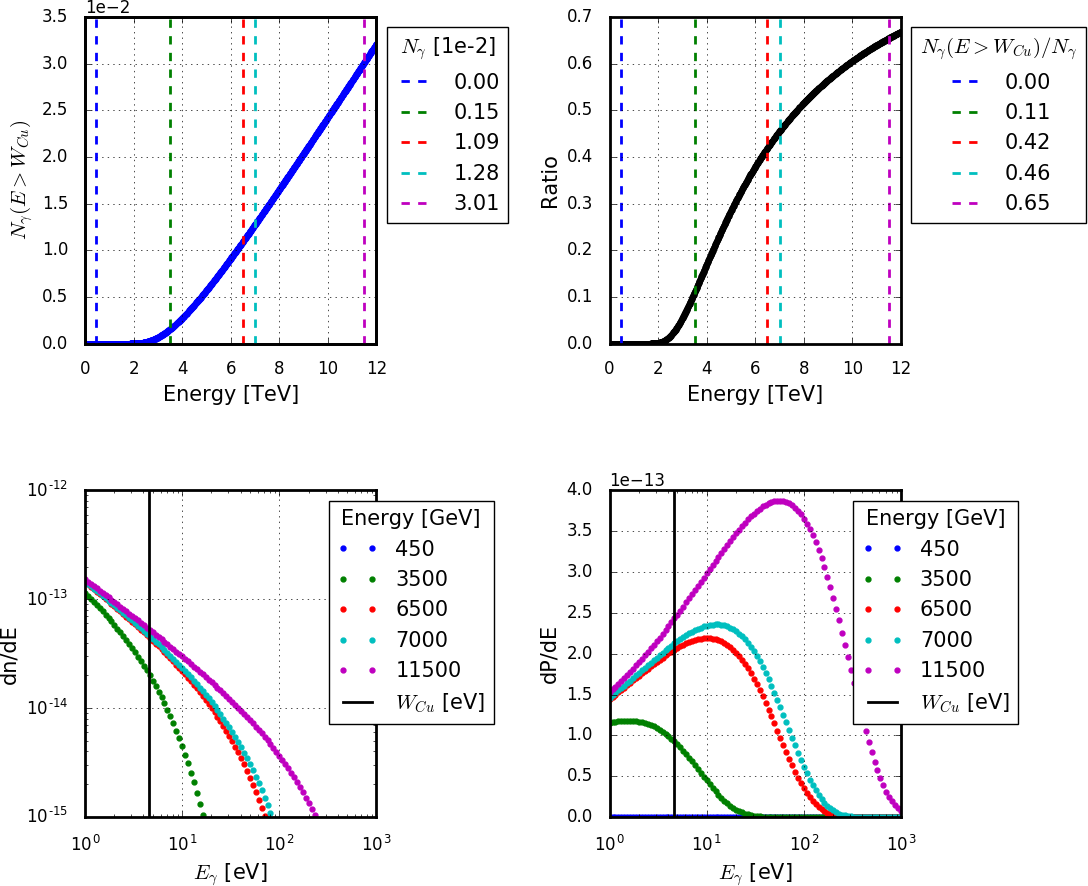
\includegraphics[width=\textwidth]{./plots/n_photons.png}
    \caption{
        Top left: Number of photons above the copper work function in the LHC.
        Top right: Ratio of photons above the copper work function.
        Bottom left: Distribution of photons for various beam energies.
        Bottom right: Energy distribution of impinging photons.
    }
    \label{fig:n_photons}
\end{figure}

